% Options for packages loaded elsewhere
% Options for packages loaded elsewhere
\PassOptionsToPackage{unicode}{hyperref}
\PassOptionsToPackage{hyphens}{url}
%
\documentclass[
  ignorenonframetext,
  aspectratio=169,
]{beamer}
\newif\ifbibliography
\usepackage{pgfpages}
\setbeamertemplate{caption}[numbered]
\setbeamertemplate{caption label separator}{: }
\setbeamercolor{caption name}{fg=normal text.fg}
\beamertemplatenavigationsymbolsempty
% remove section numbering
\setbeamertemplate{part page}{
  \centering
  \begin{beamercolorbox}[sep=16pt,center]{part title}
    \usebeamerfont{part title}\insertpart\par
  \end{beamercolorbox}
}
\setbeamertemplate{section page}{
  \centering
  \begin{beamercolorbox}[sep=12pt,center]{section title}
    \usebeamerfont{section title}\insertsection\par
  \end{beamercolorbox}
}
\setbeamertemplate{subsection page}{
  \centering
  \begin{beamercolorbox}[sep=8pt,center]{subsection title}
    \usebeamerfont{subsection title}\insertsubsection\par
  \end{beamercolorbox}
}
% Prevent slide breaks in the middle of a paragraph
\widowpenalties 1 10000
\raggedbottom
\usepackage{iftex}
\ifPDFTeX
  \usepackage[T1]{fontenc}
  \usepackage[utf8]{inputenc}
  \usepackage{textcomp} % provide euro and other symbols
\else % if luatex or xetex
  \usepackage{unicode-math} % this also loads fontspec
  \defaultfontfeatures{Scale=MatchLowercase}
  \defaultfontfeatures[\rmfamily]{Ligatures=TeX,Scale=1}
\fi
\usepackage{lmodern}

\usetheme[]{metropolis}
\ifPDFTeX\else
  % xetex/luatex font selection
\fi
% Use upquote if available, for straight quotes in verbatim environments
\IfFileExists{upquote.sty}{\usepackage{upquote}}{}
\IfFileExists{microtype.sty}{% use microtype if available
  \usepackage[]{microtype}
  \UseMicrotypeSet[protrusion]{basicmath} % disable protrusion for tt fonts
}{}
\makeatletter
\@ifundefined{KOMAClassName}{% if non-KOMA class
  \IfFileExists{parskip.sty}{%
    \usepackage{parskip}
  }{% else
    \setlength{\parindent}{0pt}
    \setlength{\parskip}{6pt plus 2pt minus 1pt}}
}{% if KOMA class
  \KOMAoptions{parskip=half}}
\makeatother


\usepackage{longtable,booktabs,array}
\usepackage{calc} % for calculating minipage widths
\usepackage{caption}
% Make caption package work with longtable
\makeatletter
\def\fnum@table{\tablename~\thetable}
\makeatother
\usepackage{graphicx}
\makeatletter
\newsavebox\pandoc@box
\newcommand*\pandocbounded[1]{% scales image to fit in text height/width
  \sbox\pandoc@box{#1}%
  \Gscale@div\@tempa{\textheight}{\dimexpr\ht\pandoc@box+\dp\pandoc@box\relax}%
  \Gscale@div\@tempb{\linewidth}{\wd\pandoc@box}%
  \ifdim\@tempb\p@<\@tempa\p@\let\@tempa\@tempb\fi% select the smaller of both
  \ifdim\@tempa\p@<\p@\scalebox{\@tempa}{\usebox\pandoc@box}%
  \else\usebox{\pandoc@box}%
  \fi%
}
% Set default figure placement to htbp
\def\fps@figure{htbp}
\makeatother





\setlength{\emergencystretch}{3em} % prevent overfull lines

\providecommand{\tightlist}{%
  \setlength{\itemsep}{0pt}\setlength{\parskip}{0pt}}



 


% ============================================================
%  Econ 2203 — Beamer Metropolis Theme Preamble
%  Course: International Trade and Policy in Agriculture
%  Instructor: Nithin M, Department of Development Economics
% ============================================================

% MUST be first: load Metropolis theme before \metroset and colour overrides
\usetheme{metropolis}

% Only load packages not already provided by pandoc's beamer template
\usepackage{amsmath,amssymb}

% ---- Brand colours -----------------------------------------
\definecolor{brandblue}{HTML}{012169}
\definecolor{brandgold}{HTML}{B9975B}
\definecolor{lightblue}{HTML}{E8EDF5}

% ---- Metropolis colour overrides ---------------------------
% Main palette
\setbeamercolor{normal text}{fg=black,bg=white}
\setbeamercolor{alerted text}{fg=brandgold}
\setbeamercolor{example text}{fg=brandblue!70!black}

% Title slide
\setbeamercolor{title}{fg=white,bg=brandblue}
\setbeamercolor{subtitle}{fg=brandgold}
\setbeamercolor{author}{fg=white}
\setbeamercolor{institute}{fg=brandgold!80!white}
\setbeamercolor{date}{fg=white}
\setbeamercolor{title page header}{fg=white,bg=brandblue}

% Frametitle bar
\setbeamercolor{frametitle}{fg=white,bg=brandblue}

% Progress bar → gold
\setbeamercolor{progress bar}{fg=brandgold,bg=brandblue!30}
\setbeamercolor{title separator}{fg=brandgold}
\setbeamercolor{progress bar in head/foot}{fg=brandgold,bg=brandblue!20}
\setbeamercolor{progress bar in section page}{fg=brandgold,bg=brandblue!20}

% Blocks
\setbeamercolor{block title}{bg=brandblue,fg=white}
\setbeamercolor{block body}{bg=lightblue,fg=black}
\setbeamercolor{block title alerted}{bg=brandgold,fg=white}
\setbeamercolor{block body alerted}{bg=brandgold!12,fg=black}
\setbeamercolor{block title example}{bg=brandblue!70!black,fg=white}
\setbeamercolor{block body example}{bg=brandblue!8,fg=black}

% Structure / lists
\setbeamercolor{structure}{fg=brandblue}
\setbeamercolor{section in toc}{fg=brandblue}
\setbeamercolor{itemize item}{fg=brandblue}
\setbeamercolor{itemize subitem}{fg=brandgold}
\setbeamercolor{enumerate item}{fg=brandblue}
\setbeamercolor{description item}{fg=brandblue}

% ---- Metropolis options ------------------------------------
\metroset{
  progressbar    = frametitle,   % gold bar under frametitle
  sectionpage    = none,
  numbering      = fraction,
  block          = fill
}

% ---- Fonts (Metropolis uses Fira Sans; fallback gracefully) -
\setbeamerfont{title}{size=\Large,series=\bfseries}
\setbeamerfont{subtitle}{size=\normalsize,series=\mdseries}
\setbeamerfont{frametitle}{size=\large,series=\bfseries}
\setbeamerfont{block title}{size=\normalsize,series=\bfseries}
\setbeamerfont{caption}{size=\footnotesize}

% ---- Footer: course info + slide number --------------------
\setbeamertemplate{footline}{%
  \begin{beamercolorbox}[wd=\paperwidth,ht=2.0ex,dp=1ex]{footline}%
    \hspace{0.8em}%
    {\footnotesize\color{brandblue!60}%
      Econ 2203 \textbar{} International Trade and Policy in Agriculture
      \hfill Nithin M \hfill
      \insertframenumber{}/\inserttotalframenumber\hspace{0.8em}}%
  \end{beamercolorbox}%
}

% ---- Misc --------------------------------------------------
\setlength{\parskip}{0.25em}
\setbeamertemplate{navigation symbols}{}

% tighter column sep for side-by-side content
\setlength{\columnsep}{0.8em}

% Fix: make \label truly robust in moving arguments (Quarto generates
% \caption{\label{fig-xxx}...} which crashes Metropolis in batchmode).
% DeclareRobustCommand creates a self-protecting robust version.
\makeatletter
\let\quarto@originallabel\label
\DeclareRobustCommand*{\label}[1]{\quarto@originallabel{#1}}
\makeatother

% Prevent figures from overflowing Beamer frames.
% width=\linewidth: scale to text width (already Quarto default);
% height=0.6\textheight: cap height so figures never push past the frame bottom.
% keepaspectratio: never distort — whichever constraint binds first wins.
\setkeys{Gin}{width=\linewidth,height=0.6\textheight,keepaspectratio}
\makeatletter
\@ifpackageloaded{caption}{}{\usepackage{caption}}
\AtBeginDocument{%
\ifdefined\contentsname
  \renewcommand*\contentsname{Table of contents}
\else
  \newcommand\contentsname{Table of contents}
\fi
\ifdefined\listfigurename
  \renewcommand*\listfigurename{List of Figures}
\else
  \newcommand\listfigurename{List of Figures}
\fi
\ifdefined\listtablename
  \renewcommand*\listtablename{List of Tables}
\else
  \newcommand\listtablename{List of Tables}
\fi
\ifdefined\figurename
  \renewcommand*\figurename{Figure}
\else
  \newcommand\figurename{Figure}
\fi
\ifdefined\tablename
  \renewcommand*\tablename{Table}
\else
  \newcommand\tablename{Table}
\fi
}
\@ifpackageloaded{float}{}{\usepackage{float}}
\floatstyle{ruled}
\@ifundefined{c@chapter}{\newfloat{codelisting}{h}{lop}}{\newfloat{codelisting}{h}{lop}[chapter]}
\floatname{codelisting}{Listing}
\newcommand*\listoflistings{\listof{codelisting}{List of Listings}}
\makeatother
\makeatletter
\makeatother
\makeatletter
\@ifpackageloaded{caption}{}{\usepackage{caption}}
\@ifpackageloaded{subcaption}{}{\usepackage{subcaption}}
\makeatother

\usepackage{bookmark}
\IfFileExists{xurl.sty}{\usepackage{xurl}}{} % add URL line breaks if available
\urlstyle{same}
\hypersetup{
  pdftitle={Lecture 11: Foreign Exchange --- Rates and Determination},
  pdfauthor={Nithin M},
  hidelinks,
  pdfcreator={LaTeX via pandoc}}


\title{Lecture 11: Foreign Exchange --- Rates and Determination}
\subtitle{Econ 2203 \textbar{} International Trade and Policy in
Agriculture}
\author{Nithin M}
\date{2026-07-04}
\institute{Department of Development Economics}

\begin{document}
\frame{\titlepage}


\begin{frame}{Foreign Exchange: Rates and Determination}
\phantomsection\label{foreign-exchange-rates-and-determination}
How the rupee's price against the dollar shapes India's agricultural
exports, food prices, and farmer incomes --- and what economic theory
tells us about why exchange rates move.
\end{frame}

\begin{frame}{What is an Exchange Rate?}
\phantomsection\label{what-is-an-exchange-rate}
\textbf{The nominal exchange rate} is the price of one currency in terms
of another.

\[e = \text{units of domestic currency per unit of foreign currency}\]

\[e_{INR/USD} = 83.5 \Rightarrow \text{1 USD costs }₹83.5\]

\begin{itemize}
\tightlist
\item
  \textbf{Direct quote} (India convention): ₹ per USD --- how many
  rupees to buy 1 dollar
\item
  \textbf{Indirect quote}: USD per ₹ --- how many dollars 1 rupee buys
  (= 1/83.5 = \$0.012)
\end{itemize}

\textbf{India 2024:} The RBI reference rate hovered near ₹83--84/USD
throughout 2024. A software exporter invoicing \$1M receives ₹83.5 crore
at spot. A food importer buying \$1M of edible oil pays ₹83.5 crore. The
same rate creates winners and losers simultaneously.
\end{frame}

\begin{frame}{Spot vs Forward Rates}
\phantomsection\label{spot-vs-forward-rates}
\begin{longtable}[]{@{}
  >{\raggedright\arraybackslash}p{(\linewidth - 4\tabcolsep) * \real{0.2647}}
  >{\raggedright\arraybackslash}p{(\linewidth - 4\tabcolsep) * \real{0.3235}}
  >{\raggedright\arraybackslash}p{(\linewidth - 4\tabcolsep) * \real{0.4118}}@{}}
\toprule\noalign{}
\begin{minipage}[b]{\linewidth}\raggedright
Feature
\end{minipage} & \begin{minipage}[b]{\linewidth}\raggedright
Spot Rate
\end{minipage} & \begin{minipage}[b]{\linewidth}\raggedright
Forward Rate
\end{minipage} \\
\midrule\noalign{}
\endhead
Settlement & Immediate (T+2) & Agreed today, settled at future date \\
Certainty & Current market price & Locked-in price for future
delivery \\
India example & ₹83.5/\$ & 3-month forward: ₹84.2/\$ \\
Use & Immediate trade settlement & Hedging future currency exposure \\
\bottomrule\noalign{}
\end{longtable}

\textbf{Forward premium calculation:}

\[\text{Forward Premium (p.a.)} = \frac{F - E}{E} \times \frac{12}{n} \times 100 = \frac{84.2 - 83.5}{83.5} \times 4 \times 100 = 3.35\%\]

\textbf{Why forward rates matter for agri exporters:} An Indian basmati
exporter signing a 3-month USD contract today faces uncertainty --- if
INR appreciates by delivery, they receive fewer rupees. By selling USD
forward at ₹84.2/\$, they lock in their revenue. The forward premium
(3.35\%) reflects market expectations of INR depreciation.
\end{frame}

\begin{frame}{Nominal vs Real Exchange Rate}
\phantomsection\label{nominal-vs-real-exchange-rate}
The \textbf{nominal} rate tells us the currency price. The \textbf{real}
rate tells us purchasing power competitiveness.

\[q = e \cdot \frac{P^*}{P}\]

where \(q\) = real exchange rate, \(e\) = nominal rate (₹/\$), \(P^*\) =
US price level, \(P\) = India price level.

\textbf{Numerical example --- Basmati Rice:}

\begin{itemize}
\tightlist
\item
  India price: ₹5,010/quintal; US equivalent: \$60/quintal; \(e\) =
  ₹83.5/\$
\item
  \(q = 83.5 \times (60/5{,}010) = 83.5 \times 0.01197 = 0.999 \approx 1\)
\item
  If India inflation pushes price to ₹5,600 with same nominal \(e\):
  \(q = 83.5 \times (60/5{,}600) = 0.894\) → INR \textbf{real
  appreciation} → Indian rice less competitive even though nominal rate
  unchanged
\end{itemize}

\textbf{Why the real rate is what matters for trade competitiveness:}
India's nominal exchange rate may be stable, but if domestic inflation
outpaces foreign inflation, Indian goods become relatively expensive.
Only a \textbf{real depreciation} --- either a nominal depreciation or
lower relative inflation --- genuinely improves export competitiveness.

\textbf{Real Effective Exchange Rate (REER):} Trade-weighted average
across all trading partners:

\[\text{REER} = \prod_i \left(e_i \cdot \frac{P_i^*}{P}\right)^{w_i}\]
\end{frame}

\begin{frame}{Appreciation vs Depreciation}
\phantomsection\label{appreciation-vs-depreciation}
\textbf{The key rule:} If \(e\) rises (more ₹ per \$) → INR
\textbf{depreciates}. If \(e\) falls → INR \textbf{appreciates}.

\begin{columns}[T]
\begin{column}{0.5\linewidth}
\begin{block}{INR Depreciation (e ↑, e.g.~₹75→₹85)}
\phantomsection\label{inr-depreciation-e-e.g.-7585}
\begin{itemize}
\tightlist
\item
  ✅ \textbf{Cotton exporters:} same USD price = more ₹ revenue
\item
  ✅ \textbf{Rice exporters (world's No.1):} Indian rice cheaper for
  foreign buyers
\item
  ✅ \textbf{Spice/marine exporters:} competitive advantage
\item
  ❌ \textbf{Edible oil importers:} same \$ price = more ₹ cost → higher
  cooking oil prices
\end{itemize}
\end{block}
\end{column}

\begin{column}{0.5\linewidth}
\begin{block}{INR Appreciation (e ↓, e.g.~₹85→₹75)}
\phantomsection\label{inr-appreciation-e-e.g.-8575}
\begin{itemize}
\tightlist
\item
  ✅ \textbf{Edible oil importers:} cheaper palm, soybean, sunflower oil
\item
  ✅ \textbf{Pulses importers:} cheaper lentils from Canada/Australia
\item
  ✅ \textbf{Fertiliser importers:} urea, DAP cheaper in ₹
\item
  ❌ \textbf{Rice exporters:} Indian rice more expensive globally →
  volume loss
\end{itemize}
\end{block}
\end{column}
\end{columns}

\note{Additional depreciation effects:

\begin{itemize}
\tightlist
\item
  ❌ \textbf{Fertiliser importers:} input costs rise → squeezes farmer
  margins
\item
  ❌ \textbf{Food inflation:} imported food basket becomes expensive
\end{itemize}

Additional appreciation effects:

\begin{itemize}
\tightlist
\item
  ✅ \textbf{Consumers:} lower food inflation
\item
  ❌ \textbf{Cotton exporters:} margins squeezed
\item
  ❌ \textbf{Spice/marine sector:} competitiveness falls
\end{itemize}}
\end{frame}

\begin{frame}{Demand for Foreign Exchange}
\phantomsection\label{demand-for-foreign-exchange}
\textbf{Who demands USD (buys USD, sells ₹)?}

\begin{itemize}
\tightlist
\item
  🛢️ \textbf{Importers} (crude oil, edible oil, electronics, machinery)
\item
  💸 \textbf{Capital outflows} (Indian firms investing abroad, FPI
  selling)
\item
  ✈️ \textbf{Tourism abroad} (Indians travelling overseas)
\item
  🏦 \textbf{Debt repayments} (external commercial borrowings in USD)
\item
  📉 \textbf{FPI outflows} (foreign portfolio investors exiting India)
\end{itemize}

\textbf{Demand function:} As \(e\) rises (INR depreciates), imports
become expensive → quantity of USD demanded falls.

\[Q_D = 216 - 2e\]

where \(e\) is ₹ per USD and \(Q\) is billions of USD. Downward-sloping
demand curve.

\textbf{Agricultural angle:} India's edible oil imports
(\textasciitilde\$14B/year) are the largest agricultural component of
USD demand --- palm oil from Indonesia/Malaysia, soybean oil from
Argentina/Brazil, sunflower oil from Ukraine. A weaker rupee makes every
litre more expensive.
\end{frame}

\begin{frame}{Supply of Foreign Exchange}
\phantomsection\label{supply-of-foreign-exchange}
\textbf{Who supplies USD (sells USD, buys ₹)?}

\begin{itemize}
\tightlist
\item
  📦 \textbf{Exporters} (IT services, rice, spices, cotton,
  pharmaceuticals) --- earn USD, convert to ₹
\item
  🏭 \textbf{FDI inflows} (foreign firms investing in India)
\item
  📈 \textbf{FPI inflows} (foreign portfolio investors buying Indian
  stocks/bonds)
\item
  💰 \textbf{Remittances} --- largest single source at
  \textasciitilde\$100B/year (\textgreater{} FDI of \$71B in FY2023)
\item
  🏦 \textbf{External borrowings} (ECBs, NRI deposits)
\end{itemize}

\textbf{Supply function:} As \(e\) rises (INR weakens), Indian exports
are cheaper globally → more exported → more USD earned and supplied.

\[Q_S = -116 + 2e\]

Upward-sloping supply curve. When \(e\) is high, each dollar of export
revenue translates to more rupees --- incentivising more exports.

\textbf{Agricultural note:} Rice (\$10B+), spices (\$4B+), cotton
(\$2B+), marine products (\$8B+) are key agri supply sources of USD. A
weak rupee boosts these exports.
\end{frame}

\begin{frame}{Foreign Exchange Market Equilibrium}
\phantomsection\label{foreign-exchange-market-equilibrium}
\begin{figure}

\centering{

\pandocbounded{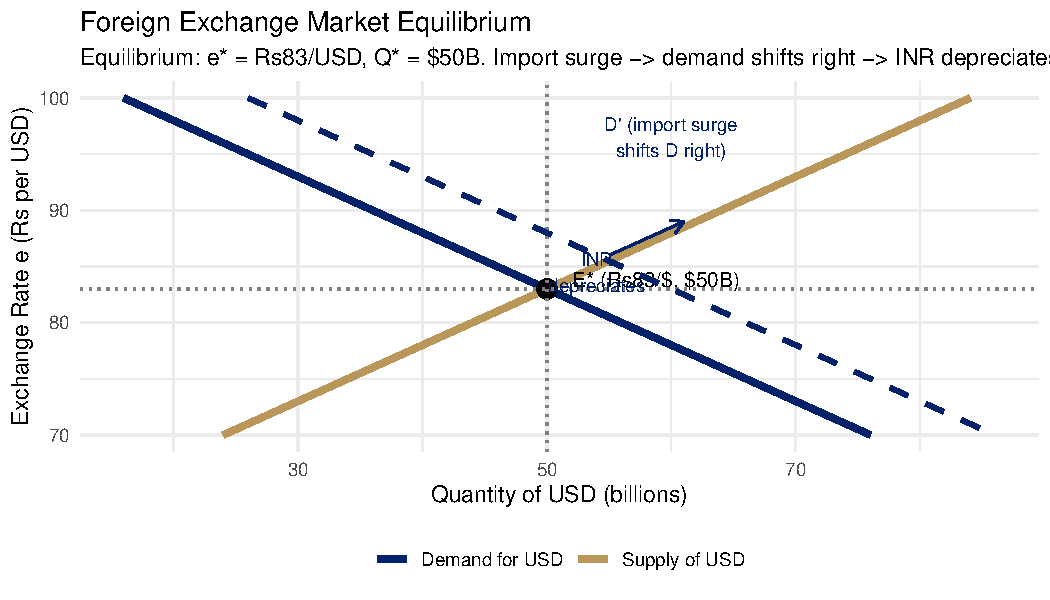
\includegraphics[keepaspectratio]{Lecture11_Foreign_Exchange_I_files/figure-beamer/fig-forex-eq-1.pdf}}

}

\caption{\label{fig-forex-eq}Foreign Exchange Market: Equilibrium
Exchange Rate Determination Source: Author's illustration.}

\end{figure}%

\textbf{Solving for equilibrium:} Set \(Q_D = Q_S\):

\[216 - 2e = -116 + 2e \Rightarrow 332 = 4e \Rightarrow e^* = 83, \quad Q^* = 50\]
\end{frame}

\begin{frame}{Factors Shifting Demand and Supply}
\phantomsection\label{factors-shifting-demand-and-supply}
\begin{longtable}[]{@{}
  >{\raggedright\arraybackslash}p{(\linewidth - 6\tabcolsep) * \real{0.2051}}
  >{\raggedright\arraybackslash}p{(\linewidth - 6\tabcolsep) * \real{0.1795}}
  >{\raggedright\arraybackslash}p{(\linewidth - 6\tabcolsep) * \real{0.4872}}
  >{\raggedright\arraybackslash}p{(\linewidth - 6\tabcolsep) * \real{0.1282}}@{}}
\toprule\noalign{}
\begin{minipage}[b]{\linewidth}\raggedright
Factor
\end{minipage} & \begin{minipage}[b]{\linewidth}\raggedright
Shift
\end{minipage} & \begin{minipage}[b]{\linewidth}\raggedright
Effect on e (₹/\$)
\end{minipage} & \begin{minipage}[b]{\linewidth}\raggedright
INR
\end{minipage} \\
\midrule\noalign{}
\endhead
India inflation ↑ & D shifts right & e ↑ & Depreciates \\
India growth ↑ → imports ↑ & D shifts right & e ↑ & Depreciates \\
FDI/FPI outflows ↑ & D shifts right & e ↑ & Depreciates \\
Oil prices ↑ & D shifts right & e ↑ & Depreciates \\
Export earnings ↑ & S shifts right & e ↓ & Appreciates \\
FDI/FPI inflows ↑ & S shifts right & e ↓ & Appreciates \\
Remittances ↑ & S shifts right & e ↓ & Appreciates \\
RBI raises rates & S shifts right (capital inflows) & e ↓ &
Appreciates \\
\bottomrule\noalign{}
\end{longtable}

\note{\textbf{Reading the table:} Every factor works through either the
\textbf{current account} (trade in goods/services) or the
\textbf{capital/financial account} (investment flows). The 2013 ``Taper
Tantrum'' combined FPI outflows (D↑) with reduced remittances to trigger
the sharpest post-2008 INR depreciation.}
\end{frame}

\begin{frame}{India INR/USD Trend (2008--2024)}
\phantomsection\label{india-inrusd-trend-20082024}
\begin{figure}

\centering{

\pandocbounded{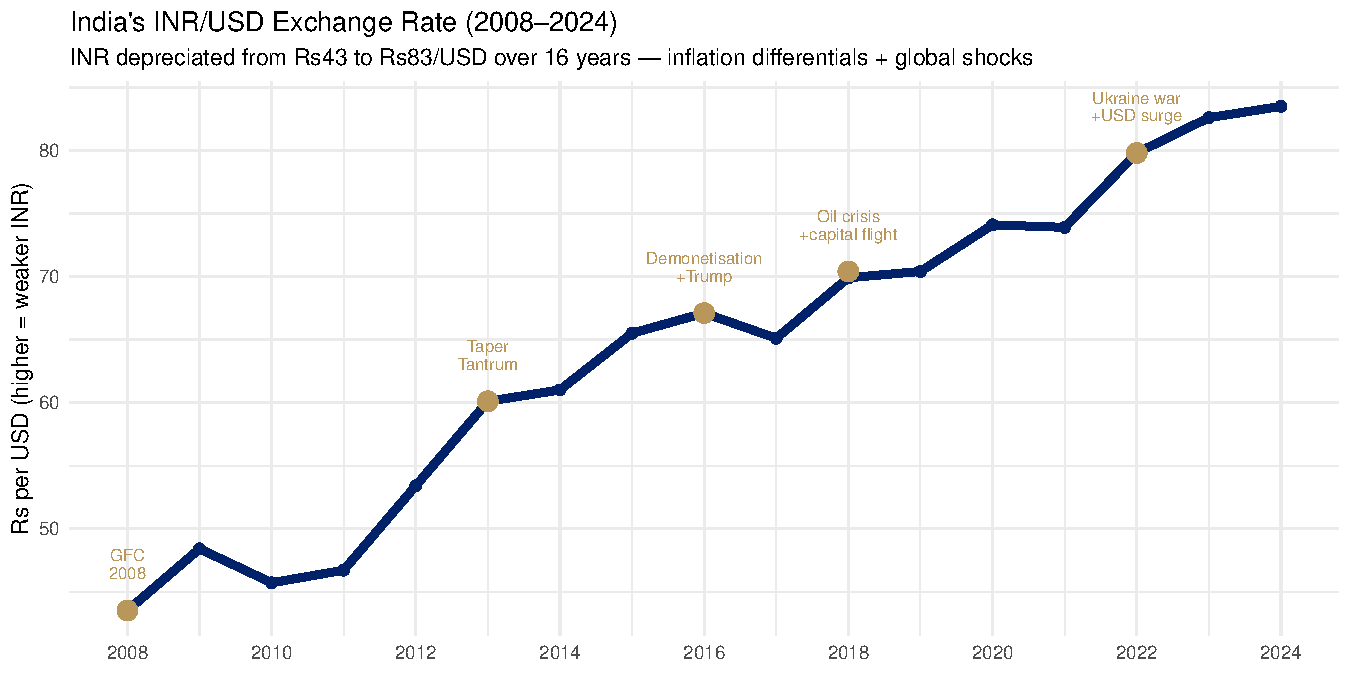
\includegraphics[keepaspectratio]{Lecture11_Foreign_Exchange_I_files/figure-beamer/fig-inr-trend-1.pdf}}

}

\caption{\label{fig-inr-trend}INR/USD Exchange Rate: Key Depreciation
Episodes (2008--2024) Source: RBI, Database on Indian Economy (DBIE).}

\end{figure}%

\begin{itemize}
\tightlist
\item
  \textbf{2008 GFC:} Global risk-off → capital flight from EMs.
  Rice/agri export demand fell; edible oil imports also dropped.
\item
  \textbf{2013 Taper Tantrum:} Fed signalled rate hike → FPI outflows.
  Cotton, rice exporters saw ₹ revenue spike but volatile.
\item
  \textbf{2018:} Iran sanctions + crude oil surge. India's \$150B crude
  import bill inflated → INR hit ₹75.
\item
  \textbf{2022 Ukraine:} Sunflower oil import disruption + USD surge →
  edible oil crisis in India.
\end{itemize}
\end{frame}

\begin{frame}{Purchasing Power Parity: Absolute PPP}
\phantomsection\label{purchasing-power-parity-absolute-ppp}
\textbf{Foundation --- Law of One Price:} In competitive markets with
free trade, identical goods sell at the same price internationally (once
converted at the exchange rate).

\textbf{Absolute PPP:} If a representative basket costs ₹4,175 in India
and \$50 in the USA:

\[e_{PPP} = \frac{P_{India}}{P_{USA}} = \frac{4175}{50} = ₹83.5 \text{ per USD}\]

\textbf{Absolute PPP says:} the exchange rate should equal the ratio of
price levels. If the actual rate differs from PPP, there is a real
misalignment.

\textbf{Big Mac Index 2024 --- Reality Check:}

\begin{longtable}[]{@{}lll@{}}
\toprule\noalign{}
Item & India & USA \\
\midrule\noalign{}
\endhead
Big Mac price & ₹259 & \$5.69 \\
Implied PPP & ₹259/\(5.69 = **₹45.5/\)** & --- \\
Actual rate & ₹83.5/\$ & --- \\
Verdict & INR \textbf{undervalued by \textasciitilde45\%} vs PPP &
--- \\
\bottomrule\noalign{}
\end{longtable}

This does not mean INR is ``wrong'' --- it reflects real structural
differences (Balassa-Samuelson effect, see Slide 13).
\end{frame}

\begin{frame}{Relative PPP}
\phantomsection\label{relative-ppp}
\textbf{Relative PPP:} Exchange rates change in proportion to inflation
differentials.

\[\% \Delta e \approx \pi_{India} - \pi_{USA}\]

\textbf{Numerical example:}

If India's inflation \(\pi_{India} = 5\%\) and USA's
\(\pi_{USA} = 2\%\):

\[\% \Delta e = 5\% - 2\% = +3\% \Rightarrow \text{INR depreciates 3\% per year}\]

\textbf{Long-run empirical test for India:}

\begin{itemize}
\tightlist
\item
  ₹45/USD (2000) → ₹83.5/USD (2024): \textbf{85.6\% depreciation} over
  24 years → \textasciitilde{}\textbf{3.5\% per year}
\item
  India avg CPI inflation (2000--2024): \textasciitilde5.5\%; US avg:
  \textasciitilde2.2\% → \textbf{differential ≈ 3.3\%}
\item
  ✓ \textbf{Broadly consistent with Relative PPP!}
\end{itemize}

\textbf{Agricultural implication:} Relative PPP predicts that India's
\textasciitilde3--4\% annual INR depreciation roughly offsets the
\textasciitilde3\% domestic cost inflation facing Indian farmers. This
means Indian agri exports maintain their global price competitiveness in
the long run --- inflation at home is offset by depreciation in the
exchange rate. Short-run deviations, however, create real competitive
swings.
\end{frame}

\begin{frame}{India: PPP-Implied vs Actual Rate}
\phantomsection\label{india-ppp-implied-vs-actual-rate}
\begin{figure}

\centering{

\pandocbounded{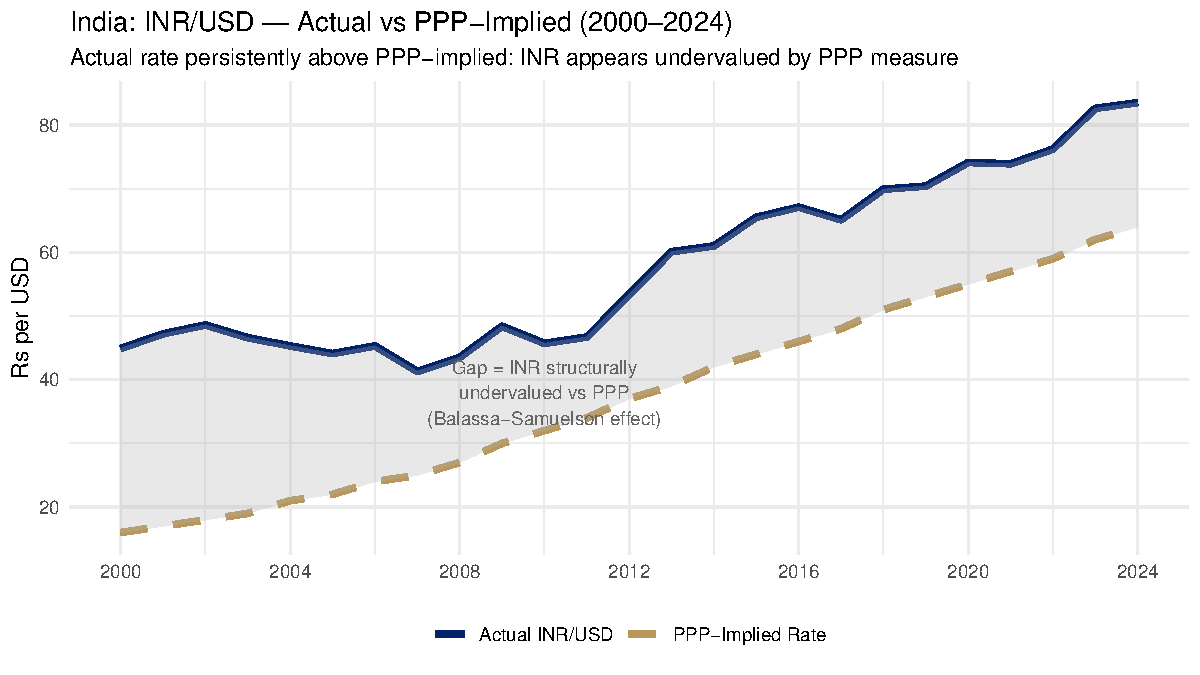
\includegraphics[keepaspectratio]{Lecture11_Foreign_Exchange_I_files/figure-beamer/fig-ppp-india-1.pdf}}

}

\caption{\label{fig-ppp-india}India: Actual Exchange Rate vs PPP-Implied
Rate (INR/USD, 2000--2024) Source: RBI; World Bank, International
Comparison Program (ICP).}

\end{figure}%

\textbf{Balassa-Samuelson Effect:} Fast-growing economies (like India)
have high productivity growth in tradables (IT, manufacturing) but not
in non-tradables (haircuts, local food). This raises wages overall,
making non-tradables expensive. PPP calculations using full CPI baskets
therefore understate the ``true'' exchange rate for a developing economy
--- the gap between actual and PPP-implied is structurally expected, not
a sign of manipulation.
\end{frame}

\begin{frame}{Limitations of PPP}
\phantomsection\label{limitations-of-ppp}
PPP is a powerful long-run benchmark but has important practical
limitations:

\begin{enumerate}
\tightlist
\item
  \textbf{Non-tradable goods} --- haircuts, education, land, local
  restaurants don't arbitrage across borders. Their prices differ
  permanently.
\item
  \textbf{Quality differences} --- a ``Big Mac'' in Tokyo ≠ a Big Mac in
  Delhi in quality perception.
\item
  \textbf{Trade barriers} --- tariffs, quotas, and transport costs
  prevent price equalisation even for tradables.
\item
  \textbf{Balassa-Samuelson effect} --- richer/faster-growing countries
  systematically have currencies above PPP because productivity gains in
  tradables spill over to raise wages in non-tradables.
\item
  \textbf{Short-run irrelevance} --- capital flows, sentiment, and
  central bank intervention dominate short-run exchange rates. PPP
  explains long-run trends, not day-to-day movements.
\end{enumerate}

\textbf{Agricultural implication:} Agricultural commodities --- rice,
wheat, cotton, edible oils, spices --- ARE tradable goods. PPP-based
analysis is therefore more applicable to food prices than to services
prices. When the IMF/World Bank assess food affordability across
countries, they use PPP-adjusted incomes. India's apparent INR
undervaluation by PPP helps explain why Indian agricultural exports are
consistently price-competitive globally.
\end{frame}

\begin{frame}{Interest Rate Parity: Uncovered IRP}
\phantomsection\label{interest-rate-parity-uncovered-irp}
\textbf{Setup:} An Indian investor has ₹1 crore to invest for 1 year.
Two options:

\begin{enumerate}
\tightlist
\item
  \textbf{INR bond} earning \(i_{India} = 7\%\) → get ₹1.07 crore in 1
  year
\item
  \textbf{USD bond} earning \(i_{USA} = 5\%\), but must convert ₹ to \$
  now and \$ back to ₹ later
\end{enumerate}

\textbf{Uncovered Interest Rate Parity (UIP):} In equilibrium, expected
returns must be equal:

\[i_{India} = i_{USA} + \frac{E^e - E}{E}\]

where \(E^e\) = expected future exchange rate (uncertain --- hence
``uncovered'').

\textbf{Rearranged:}

\[\frac{E^e - E}{E} = i_{India} - i_{USA} = 7\% - 5\% = 2\%\]

→ Market expects INR to \textbf{depreciate 2\% per year} to equalise
returns.

\textbf{Interpretation:} India's higher interest rates do NOT simply
attract unlimited capital inflows --- because investors price in the
expected currency depreciation. The interest rate advantage is exactly
offset (in equilibrium) by the expected loss from holding a depreciating
currency. This is why India cannot run 8\% rates indefinitely without
currency pressure.
\end{frame}

\begin{frame}{UIP Diagram}
\phantomsection\label{uip-diagram}
\begin{figure}

\centering{

\pandocbounded{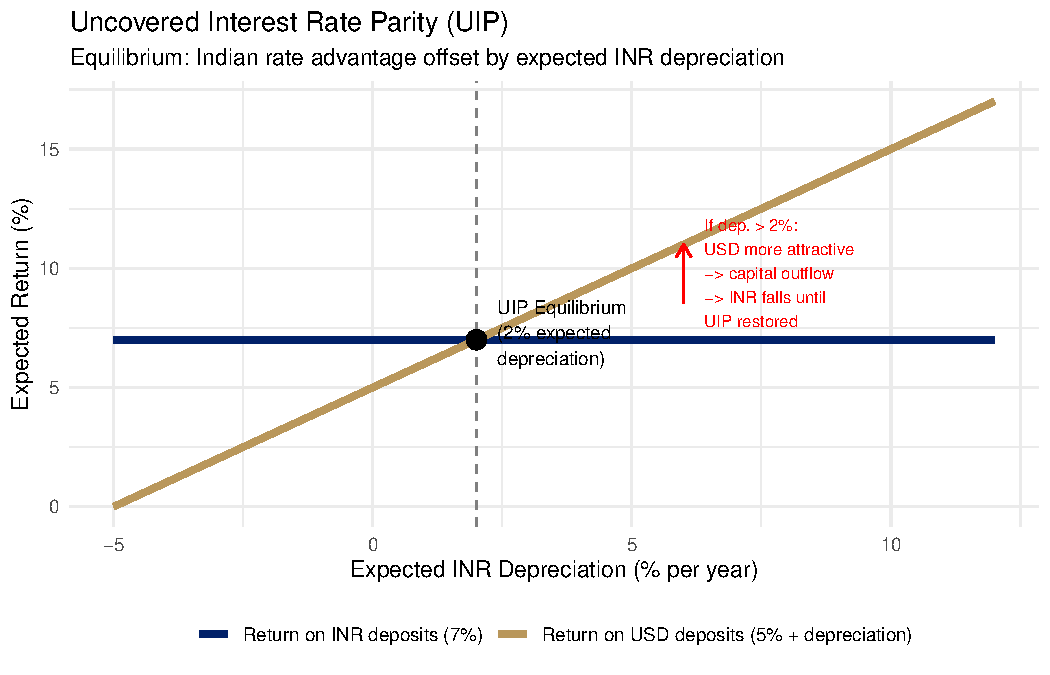
\includegraphics[keepaspectratio]{Lecture11_Foreign_Exchange_I_files/figure-beamer/fig-irp-1.pdf}}

}

\caption{\label{fig-irp}Uncovered Interest Rate Parity: Expected Return
Equalization Source: Author's illustration.}

\end{figure}%
\end{frame}

\begin{frame}{Covered vs Uncovered IRP}
\phantomsection\label{covered-vs-uncovered-irp}
\textbf{Covered Interest Rate Parity (CIP):} Uses the \emph{forward}
exchange rate --- no uncertainty.

\[i_{India} = i_{USA} + \frac{F - E}{E}\]

where \(F\) = forward exchange rate (agreed today, settled at future
date --- no currency risk).

\textbf{Uncovered Interest Rate Parity (UIP):} Uses the \emph{expected
future spot} rate --- uncertain.

\[i_{India} = i_{USA} + \frac{E^e - E}{E}\]

\textbf{Empirical verdict:}

\begin{itemize}
\tightlist
\item
  \textbf{CIP} holds almost perfectly in practice --- arbitrage desks
  enforce it millisecond-to-millisecond.
\item
  \textbf{UIP} weaker empirically --- exchange rate risk premium and
  investor irrationality cause deviations.
\end{itemize}

\textbf{Numerical CIP check (India, 2024):}

\begin{itemize}
\tightlist
\item
  Spot \(E\) = ₹83.5/\$; 3-month forward \(F\) = ₹84.2/\$
\item
  Forward premium = \((84.2-83.5)/83.5 \times 4 \times 100 = 3.35\%\)
  p.a.
\item
  Interest differential: \(i_{India}=6.5\%\), \(i_{USA}=5.3\%\) →
  \(\Delta i = 1.2\%\)
\item
  Gap (3.35\% vs 1.2\%) is explained by \textbf{country risk premium} on
  Indian sovereign debt.
\end{itemize}

\textbf{Agri exporter hedging via CIP:} A rice exporter expecting
\(5M in 6 months sells USD forward at ₹84.2/\). CIP guarantees the
forward rate is fairly priced relative to the interest differential ---
no ``free money'' from hedging, but the exporter eliminates revenue
uncertainty. The forward premium (3.35\%) is the cost of certainty.
\end{frame}

\begin{frame}{RBI Intervention in the Forex Market}
\phantomsection\label{rbi-intervention-in-the-forex-market}
\textbf{How RBI intervenes:}

\begin{itemize}
\tightlist
\item
  \textbf{Preventing excessive depreciation:} RBI \emph{sells} USD from
  reserves → increases USD supply in market → reduces e (strengthens
  INR)
\item
  \textbf{Preventing excessive appreciation:} RBI \emph{buys} USD →
  reduces USD supply → increases e (weakens INR)
\end{itemize}

\begin{columns}[T]
\begin{column}{0.55\linewidth}
\textbf{Sterilisation mechanism:}

When RBI buys USD (injects ₹ into economy): 1. Buy USD → ₹ liquidity
increases (inflationary) 2. Simultaneously \emph{sell} government
securities (G-secs) → absorbs ₹ back 3. Net effect: money supply
\emph{neutral}, but forex reserves increase

\textbf{India's forex reserve trajectory:}

\begin{longtable}[]{@{}lll@{}}
\toprule\noalign{}
Year & Reserves & Import cover \\
\midrule\noalign{}
\endhead
1991 & \$1.2B & 2 weeks (\textbf{crisis}) \\
2004 & \$113B & \textasciitilde12 months \\
2014 & \$304B & \textasciitilde8 months \\
2024 & \textasciitilde\$645B & \textasciitilde11 months \\
\bottomrule\noalign{}
\end{longtable}
\end{column}

\begin{column}{0.45\linewidth}
\textbf{Sterilisation and agriculture:}

When RBI sterilises USD purchases: - G-sec yields are kept from falling
- Domestic interest rates remain higher - This keeps credit costs for
agri sector elevated

RBI's twin mandate --- currency stability + price stability --- creates
a constant tension in agri credit markets.

\textbf{India is NOT classified} as a currency manipulator by the US
Treasury --- interventions are two-sided and RBI has intervened in both
directions over 2022--2024.
\end{column}
\end{columns}
\end{frame}

\begin{frame}{Determinants Summary Table}
\phantomsection\label{determinants-summary-table}
\begin{longtable}[]{@{}llll@{}}
\toprule\noalign{}
Factor & Channel & Effect on e (₹/\$) & INR Direction \\
\midrule\noalign{}
\endhead
India inflation ↑ & PPP/competitiveness & e ↑ & Depreciates \\
India growth ↑ → imports ↑ & Current account & e ↑ & Depreciates \\
FDI/FPI outflows ↑ & Capital account & e ↑ & Depreciates \\
Oil prices ↑ (India imports 85\%) & Import demand & e ↑ & Depreciates \\
US Fed raises rates & Carry trade reversal & e ↑ & Depreciates \\
Remittances ↑ & Capital inflows & e ↓ & Appreciates \\
RBI raises repo rate & Capital inflows & e ↓ & Appreciates \\
Export boom (rice, IT) & Current account & e ↓ & Appreciates \\
\bottomrule\noalign{}
\end{longtable}

\note{\textbf{Agricultural angle:} Oil price channel is critical ---
India imports 85\% of crude oil. Every \$10/barrel rise in oil adds
\textasciitilde\$15B to the import bill, directly pressuring INR. The
2022 Ukraine war triggered this simultaneously with sunflower oil supply
disruption --- a double agricultural shock transmitted through the forex
market.}
\end{frame}

\begin{frame}{Implications for Agricultural Trade}
\phantomsection\label{implications-for-agricultural-trade}
\begin{columns}[T]
\begin{column}{0.5\linewidth}
\textbf{Depreciation (e ↑: ₹75→₹85)}

\emph{Winners --- Exporters:}

\begin{itemize}
\tightlist
\item
  🌾 Rice (\textasciitilde\$10B/yr): world's No.1 exporter;
  \textasciitilde10.7\% cheaper for importers
\item
  🌶️ Spices (\textasciitilde\$4B/yr): highly price-elastic globally
\item
  🐟 Marine products (\textasciitilde\$8B/yr): shrimp, fish more
  competitive
\item
  🌿 Cotton (\textasciitilde\$2B/yr): textile exporters gain
\end{itemize}

\emph{Losers --- Input costs rise:}

\begin{itemize}
\tightlist
\item
  🧪 Fertiliser imports (urea, DAP) cost more
\item
  🛢️ Diesel for tractors/pumps more expensive
\end{itemize}
\end{column}

\begin{column}{0.5\linewidth}
\textbf{Appreciation (e ↓: ₹85→₹75)}

\emph{Winners --- Importers/Consumers:}

\begin{itemize}
\tightlist
\item
  🫙 Edible oils (\$14B+/yr): cheaper cooking oil for consumers
\item
  🌱 Pulses (\$3B+/yr): cheaper lentils, chickpeas
\item
  🧪 Fertilisers: urea, DAP, MOP cheaper in ₹ terms
\end{itemize}

\emph{Losers --- Exporters squeezed:}

\begin{itemize}
\tightlist
\item
  Rice, spice, marine, cotton exporters lose margin
\end{itemize}
\end{column}
\end{columns}
\end{frame}

\begin{frame}{Exchange Rate: The Policy Tension}
\phantomsection\label{exchange-rate-the-policy-tension}
\textbf{RBI's dilemma for agricultural trade:}

\begin{itemize}
\tightlist
\item
  Defending INR → helps consumers (lower food inflation) but hurts agri
  exporters
\item
  Allowing depreciation → helps exporters but risks food inflation
  spiral
\end{itemize}

India's response: simultaneously subsidise fertilisers (mitigate input
cost channel) \textbf{and} impose rice export bans (protect domestic
supply) --- policies that interact with the exchange rate in complex
ways.
\end{frame}

\begin{frame}{Key Takeaways}
\phantomsection\label{key-takeaways}
\textbf{Six core concepts from Lecture 11:}

\begin{enumerate}
\item
  \textbf{Exchange rate notation:} \(e = ₹/USD\); higher \(e\) = weaker
  INR (depreciation); lower \(e\) = stronger INR (appreciation)
\item
  \textbf{Market equilibrium:} \(Q_D(e) = Q_S(e)\) determines \(e^*\);
  shifts from trade and capital flows move equilibrium. Solving:
  \(216-2e = -116+2e \Rightarrow e^* = 83\)
\item
  \textbf{Real exchange rate} \(q = e \cdot P^*/P\): only real
  depreciation --- not just nominal --- genuinely improves export
  competitiveness. REER is the trade-weighted measure RBI monitors.
\item
  \textbf{Absolute PPP:} \(e_{PPP} = P/P^*\); India's actual rate
  \textgreater\textgreater{} PPP (Balassa-Samuelson); \textbf{Relative
  PPP:} \(\Delta e \approx \pi - \pi^*\) --- \textasciitilde3--4\%
  annual INR depreciation predicted and observed over 2000--2024.
\item
  \textbf{Interest Rate Parity (UIP):}
  \(i_{India} - i_{USA} = (E^e - E)/E\); India's higher rates are offset
  by expected depreciation --- no free lunch from the interest
  differential.
\item
  \textbf{Agriculture:} depreciation boosts rice/cotton/spice exports;
  raises edible oil/fertiliser import costs --- a constant policy
  tension that explains India's oscillation between export bans and
  import duty waivers.
\end{enumerate}
\end{frame}

\begin{frame}{Next Lecture: Exchange Rate Systems and Open Economy
Macroeconomics}
\phantomsection\label{next-lecture-exchange-rate-systems-and-open-economy-macroeconomics}
\begin{columns}[T]
\begin{column}{0.6\linewidth}
\textbf{Lecture 12 (July 11, 2026):}

\emph{Forex Market --- Exchange Rate Systems and Open Economy Macro}

We will cover:

\begin{itemize}
\tightlist
\item
  Fixed vs floating vs managed exchange rate systems
\item
  The Impossible Trinity (Mundell trilemma)
\item
  Mundell-Fleming model: IS-LM-BP

  \begin{itemize}
  \tightlist
  \item
    Fiscal and monetary policy effectiveness under different regimes
  \end{itemize}
\item
  RBI's managed float in practice
\item
  India's forex reserves: from crisis to abundance
\item
  Forward market and currency hedging
\item
  Exchange rate pass-through to agricultural prices
\end{itemize}
\end{column}

\begin{column}{0.4\linewidth}
\textbf{Bridge from today:}

Today we learned \emph{how} the rupee rate is determined by
supply/demand, PPP, and interest rate parity.

Next lecture we study:

\begin{itemize}
\tightlist
\item
  What \emph{system} India operates under
\item
  How government \textbf{policy} affects the exchange rate
\item
  How open-economy \textbf{macroeconomics} links monetary policy, fiscal
  policy, and the exchange rate
\end{itemize}

\emph{Reading: Salvatore Ch 14-15; Appleyard Ch 20-21}
\end{column}
\end{columns}
\end{frame}

\section{Appendix}\label{appendix}

\begin{frame}{Additional Resources}
\phantomsection\label{additional-resources}
\begin{columns}[T]
\begin{column}{0.5\linewidth}
\textbf{Further Reading}

\begin{itemize}
\tightlist
\item
  \emph{International Economics} --- Salvatore (Ch. 15-16)
\item
  \emph{International Economics} --- Appleyard \& Field (Ch. 15-16)
\item
  RBI/DGCI\&S/APEDA databases for latest data
\end{itemize}
\end{column}

\begin{column}{0.5\linewidth}
\textbf{Key Data Sources}

\begin{itemize}
\tightlist
\item
  DGCI\&S: India's merchandise trade
\item
  RBI: Balance of payments data\\
\item
  APEDA: Agricultural export statistics
\item
  WTO: Tariff and trade databases
\end{itemize}
\end{column}
\end{columns}
\end{frame}




\end{document}
